%%%%%%%%%%%%%%%%%%%%%%%%%%%%%%%%%%%%%%%%%%%%%%%%%%%%%%%%%%%%%%%%%%%%%%%%%%%%%%%%%%%%%%%%%%%%%%%%%%%%%%%%%%%%%%%%%%%%%%%%%%%%%%%%%%%
\paragraph{Beschleunigte Bewegung}

Ihr saßt bestimmt schon mal in einem Auto. Der Autor hatte neulich das Vergnügen, einen Elektroauto mit einem richtig starken Motor zu fahren -- so stark, dass es einen in den Sitz drückt und man das Gefühl hat: jemand hat mich am Sitz festgeklebt. Dieses Gefühl, in den Sitz gedrückt zu werden wenn die Geschwindigkeit zunimmt, nennt man -- es wird Euch nicht überraschen: Beschleunigung. Ihr kennt aber auch bestimmt das Gegenteil: das Auto wird so sehr abgebremst, dass man das Gefühl hat, nach vorne zu fliegen und man nur vom Gurt festegehalten wird. Nun die Überraschung: für den Physiker ist das auch Beschleunigung, nur eben in die entgegengesetze Richtung. Ihr könnt Euch das so vorstellen: das Auto steht an einem Hang und rollt rückwärts. Wenn man nun Gas gibt, wird es erst langsamer, kommt zum Stillstand und fährt dann schließlich nach vorne, den Berg hoch. Wie Ihr im vorhergehenden Abschnitt schon gesehen habt, ist es wichtig, den Bezugspunkt zu wählen -- aber auch die Richtung: auch die Beschleunigung kann ``negativ'' sein, abhängig davon, in welche Richtung sieht wirkt. 

Für die beschleunigte Bewegung gibt es zwei wichtige Gleichungen:
\begin{align}
    v(t) &= v_0 + a\cdot t \\
    s(t) &= s_0 + \frac12 a\cdot t^2 \,.
\end{align}
Hier sind $v_0$ und $s_0$ die anfängliche Geschwindigkeit und Strecke, $a$ die Beschleunigung und wieder $t$ die Zeit.\footnote{%
    Diese Variablennamen kommen aus dem Lateinischen, \emph{acceleratio} für Beschleunigung und \emph{gravitas} (Schwere) für Erdbeschleunigung. Im Englischen benutzt man \emph{acceleration} und \emph{gravity}.}
Im vorhergehenden Abschnitt haben wir ja gesehen, dass Objekte auf der Erde durch die Erdanziehung in Richtung Erde beschleunigt werden. Die Beschleunigung, die auf eine Tropfen wirkt, ist die Erdbeschleunigung, die durch $g$ beschrieben wird. Diese Erdbeschleunigung\footnote{%
    Die Kraft, mit der ein Objekt angezogen wird, nennt man ganz allgemein Gravitation. Alle Objekt -- die Masse haben -- ziehen sich durch Gravitation an. Erstaunlicherweise sind sich die Physiker noch nicht im Klaren, was Gravitation tatsächlich ist. Das gilt übrigens auch in anderen Bereichen, in denen Physiker Dinge zwar sehr genau mathematisch beschreiben und berechnen können -- den Ursache dafür aber noch nicht kennen. Der Autor möchte zu Gravitation auch anmerken, dass eine Gruppe Mathematiker 2026 darstellen konnte, dass -- entgegen bisheriger Lehrmeinung -- die Gravition keine Grundkraft ist.}
    % FIXME maybe too much for kids ("Grundkraft"), evtl. Studio weglassen
ist (fast) eine Konstante, die wir mit $g = \qty{9,81}{\meter\per\second^2}$ verwenden können.

Um herauszufinden, was es bedeutet, wenn ein Körper zur Erde fällt betrachten wir ein Sandkorn. Starke Winde können den Sand der Sahara über Hunderte Kilometer weit  bis zu einer Höhe von \qty{10}{\km} um die Erde tragen (der Autor hat diesen roten Sand schon in seiner Kindheit in Deutschland zur Erde fallen sehen). 
% TODO vll. Fußnote über "jet streams"
Wenn ein Sandkorn nun aus dieser Höhe mit fällt, beschrieben durch die genannten Formeln, machen wir einigen aufschlussreiche Feststellungen.
\begin{figure}[h]
    % GNUPLOT: LaTeX picture with Postscript
\begingroup
  \makeatletter
  \providecommand\color[2][]{%
    \GenericError{(gnuplot) \space\space\space\@spaces}{%
      Package color not loaded in conjunction with
      terminal option `colourtext'%
    }{See the gnuplot documentation for explanation.%
    }{Either use 'blacktext' in gnuplot or load the package
      color.sty in LaTeX.}%
    \renewcommand\color[2][]{}%
  }%
  \providecommand\includegraphics[2][]{%
    \GenericError{(gnuplot) \space\space\space\@spaces}{%
      Package graphicx or graphics not loaded%
    }{See the gnuplot documentation for explanation.%
    }{The gnuplot epslatex terminal needs graphicx.sty or graphics.sty.}%
    \renewcommand\includegraphics[2][]{}%
  }%
  \providecommand\rotatebox[2]{#2}%
  \@ifundefined{ifGPcolor}{%
    \newif\ifGPcolor
    \GPcolortrue
  }{}%
  \@ifundefined{ifGPblacktext}{%
    \newif\ifGPblacktext
    \GPblacktexttrue
  }{}%
  % define a \g@addto@macro without @ in the name:
  \let\gplgaddtomacro\g@addto@macro
  % define empty templates for all commands taking text:
  \gdef\gplbacktext{}%
  \gdef\gplfronttext{}%
  \makeatother
  \ifGPblacktext
    % no textcolor at all
    \def\colorrgb#1{}%
    \def\colorgray#1{}%
  \else
    % gray or color?
    \ifGPcolor
      \def\colorrgb#1{\color[rgb]{#1}}%
      \def\colorgray#1{\color[gray]{#1}}%
      \expandafter\def\csname LTw\endcsname{\color{white}}%
      \expandafter\def\csname LTb\endcsname{\color{black}}%
      \expandafter\def\csname LTa\endcsname{\color{black}}%
      \expandafter\def\csname LT0\endcsname{\color[rgb]{1,0,0}}%
      \expandafter\def\csname LT1\endcsname{\color[rgb]{0,1,0}}%
      \expandafter\def\csname LT2\endcsname{\color[rgb]{0,0,1}}%
      \expandafter\def\csname LT3\endcsname{\color[rgb]{1,0,1}}%
      \expandafter\def\csname LT4\endcsname{\color[rgb]{0,1,1}}%
      \expandafter\def\csname LT5\endcsname{\color[rgb]{1,1,0}}%
      \expandafter\def\csname LT6\endcsname{\color[rgb]{0,0,0}}%
      \expandafter\def\csname LT7\endcsname{\color[rgb]{1,0.3,0}}%
      \expandafter\def\csname LT8\endcsname{\color[rgb]{0.5,0.5,0.5}}%
    \else
      % gray
      \def\colorrgb#1{\color{black}}%
      \def\colorgray#1{\color[gray]{#1}}%
      \expandafter\def\csname LTw\endcsname{\color{white}}%
      \expandafter\def\csname LTb\endcsname{\color{black}}%
      \expandafter\def\csname LTa\endcsname{\color{black}}%
      \expandafter\def\csname LT0\endcsname{\color{black}}%
      \expandafter\def\csname LT1\endcsname{\color{black}}%
      \expandafter\def\csname LT2\endcsname{\color{black}}%
      \expandafter\def\csname LT3\endcsname{\color{black}}%
      \expandafter\def\csname LT4\endcsname{\color{black}}%
      \expandafter\def\csname LT5\endcsname{\color{black}}%
      \expandafter\def\csname LT6\endcsname{\color{black}}%
      \expandafter\def\csname LT7\endcsname{\color{black}}%
      \expandafter\def\csname LT8\endcsname{\color{black}}%
    \fi
  \fi
    \setlength{\unitlength}{0.0500bp}%
    \ifx\gptboxheight\undefined%
      \newlength{\gptboxheight}%
      \newlength{\gptboxwidth}%
      \newsavebox{\gptboxtext}%
    \fi%
    \setlength{\fboxrule}{0.5pt}%
    \setlength{\fboxsep}{1pt}%
    \definecolor{tbcol}{rgb}{1,1,1}%
\begin{picture}(6800.00,4520.00)%
    \gplgaddtomacro\gplbacktext{%
      \colorrgb{0.12,0.47,0.71}%%
      \put(812,697){\makebox(0,0)[r]{\strut{}$0$}}%
      \colorrgb{0.12,0.47,0.71}%%
      \put(812,1380){\makebox(0,0)[r]{\strut{}$2000$}}%
      \colorrgb{0.12,0.47,0.71}%%
      \put(812,2062){\makebox(0,0)[r]{\strut{}$4000$}}%
      \colorrgb{0.12,0.47,0.71}%%
      \put(812,2745){\makebox(0,0)[r]{\strut{}$6000$}}%
      \colorrgb{0.12,0.47,0.71}%%
      \put(812,3428){\makebox(0,0)[r]{\strut{}$8000$}}%
      \colorrgb{0.12,0.47,0.71}%%
      \put(812,4111){\makebox(0,0)[r]{\strut{}$10000$}}%
      \csname LTb\endcsname%%
      \put(904,479){\makebox(0,0){\strut{}$0$}}%
      \csname LTb\endcsname%%
      \put(1889,479){\makebox(0,0){\strut{}$10$}}%
      \csname LTb\endcsname%%
      \put(2874,479){\makebox(0,0){\strut{}$20$}}%
      \csname LTb\endcsname%%
      \put(3859,479){\makebox(0,0){\strut{}$30$}}%
      \csname LTb\endcsname%%
      \put(4844,479){\makebox(0,0){\strut{}$40$}}%
      \csname LTb\endcsname%%
      \put(5830,479){\makebox(0,0){\strut{}$50$}}%
      \colorrgb{0.84,0.15,0.16}%%
      \put(5921,697){\makebox(0,0)[l]{\strut{}$0$}}%
      \colorrgb{0.84,0.15,0.16}%%
      \put(5921,1414){\makebox(0,0)[l]{\strut{}$100$}}%
      \colorrgb{0.84,0.15,0.16}%%
      \put(5921,2131){\makebox(0,0)[l]{\strut{}$200$}}%
      \colorrgb{0.84,0.15,0.16}%%
      \put(5921,2848){\makebox(0,0)[l]{\strut{}$300$}}%
      \colorrgb{0.84,0.15,0.16}%%
      \put(5921,3565){\makebox(0,0)[l]{\strut{}$400$}}%
      \colorrgb{0.84,0.15,0.16}%%
      \put(5921,4282){\makebox(0,0)[l]{\strut{}$500$}}%
    }%
    \gplgaddtomacro\gplfronttext{%
      \csname LTb\endcsname%%
      \put(5102,4085){\makebox(0,0)[r]{\strut{}Höhe}}%
      \csname LTb\endcsname%%
      \put(5102,3868){\makebox(0,0)[r]{\strut{}Geschwindigkeit}}%
      \csname LTb\endcsname%%
      \put(5102,3650){\makebox(0,0)[r]{\strut{}Schallmauer}}%
      \colorrgb{0.12,0.47,0.71}%%
      \put(177,2489){\rotatebox{-270.00}{\makebox(0,0){\strut{}Höhe h [m]}}}%
      \colorrgb{0.84,0.15,0.16}%%
      \put(6396,2489){\rotatebox{-270.00}{\makebox(0,0){\strut{}Geschwindigkeit v [m/s]}}}%
      \csname LTb\endcsname%%
      \put(3367,152){\makebox(0,0){\strut{}Zeit t [s]}}%
    }%
    \gplbacktext
    \put(0,0){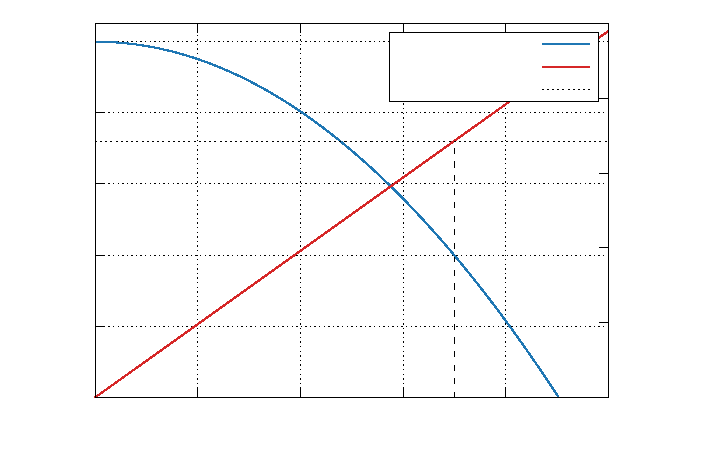
\includegraphics[width={340.00bp},height={226.00bp}]{images/physik/freierfall}}%
    \gplfronttext
  \end{picture}%
\endgroup

    \caption{Der freie Fall eines Sandkorns aus 10 km Höhe (ohne Luftwiderstand). Die blaue Linie zeigt die Höhe, die rote Linie die Geschwindigkeit. Nach etwa 35 Sekunden (gestrichelte Linie) durchbricht das Sandkorn die Schallmauer (gepunktete Linie).}
    \label{fig:physik:bewegung:sandkorn}
\end{figure}
Die Flugstrecke und Geschwindigkeit dieses Sandkorns werden in Abb.~\ref{fig:physik:bewegung:sandkorn} gezeigt. Da sehen wir, dass das Sandkorn nach etwa \qty{35}{s} die Schallmauer durchbricht (um die \qty{1200}{\km\per\hour}) und schon \qty{6}{\km} weit geflogen ist. Nach \qty{45}{\second} schlägt es dann mit eine Geschwindigkeit von etwa \qty{1620}{\km\per\hour} auf den Boden. 
% TODO explain that we're suddenly dealing with a graph with two axes!

Solch eine Geschwindigkeit würde selbst für ein Sandkorn zu schweren Verletzungen führen -- in der Realität wird ein Sandkorn aber höchstens mit \qty{15}{\km\per\hour} zu Boden fallen, denn die obigen Formeln haben einen ``kleinen'' Nachteil: sie gelten nur im Vakuum, also ohne Luftreibung. Da wir später aber unser ``Regensimulation'' zu programmieren wollen, dass sie natürlich aussieht, müssen wir uns mit dem Thema Reibung befassen.
